\begin{solution}[label=ques:4a]
  \begin{question}
    Without using any measurements, create a quantum circuit that maps $\ket{00}$ to $\frac{1}{\sqrt{2}}(\ket{01} - \ket{10})$.
  \end{question}
  \tcblower{}
  \begin{proof}[Solution]
    Consider the following quantum circuit,

    \begin{minipage}[t]{\textwidth}
      \centering
      \begin{quantikz}
        \lstick{$\ket{0}$} & \gate{X} & \gate{H} & \ctrl{1} & \qw\\
        \lstick{$\ket{0}$} & \gate{X} & \qw & \targ{} & \qw
      \end{quantikz}
    \end{minipage}

    This circuit maps $\ket{00}$ to $\frac{1}{\sqrt{2}}(\ket{01} - \ket{10})$.
  \end{proof}
\end{solution}

\begin{solution}[label=ques:4b]
  \begin{question}
    Create the circuit (with measurements added to both qubits) within the IBM Q Experience. Run it on a quantum computer. Again, include a screenshot of the results.

Hopefully, this gives you a nice introduction to IBM Q. There are other software suites available online, but this may be the most convenient. In the future, if you're struggling with analyzing a quantum circuit, you might use this as a tool.
  \end{question}
  \tcblower{}
  \begin{proof}[Solution]
    The quantum circuit was created in the IBM Quantum Composer and run on the IBM Q Experience. The results are shown in Figure~\ref{fig:4b_sv} and Figure~\ref{fig:4b_sb}.\par
    \begin{minipage}[t]{\textwidth}
      \centering
      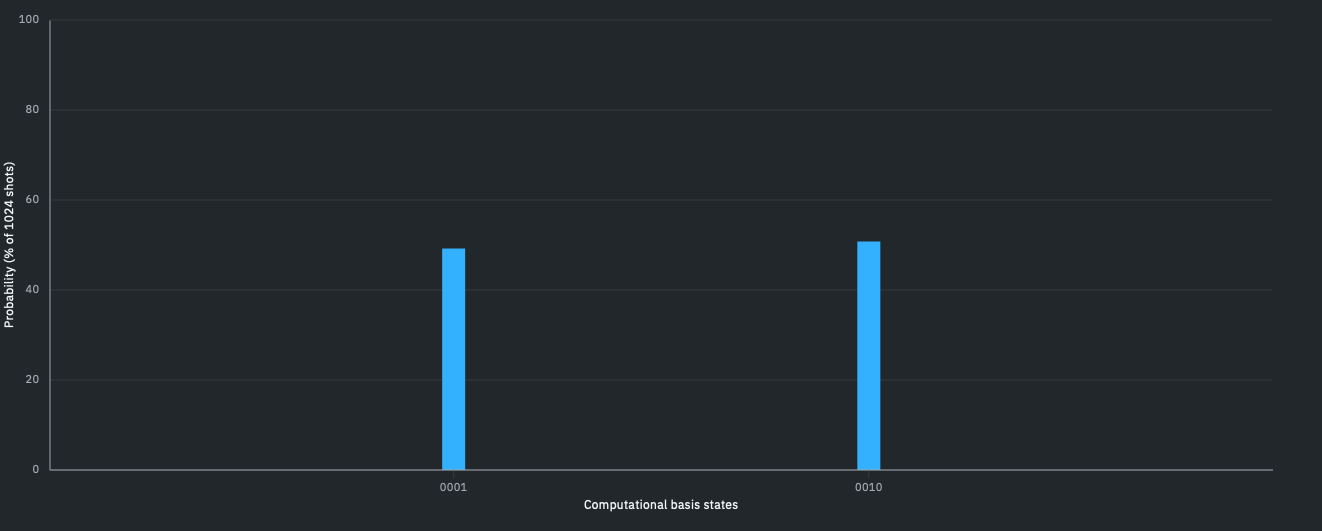
\includegraphics[width=0.66\textwidth]{q4_b_sv.png}
      \captionof{figure}{Screenshot of the results from the IBM Quantum Composer for statevector simulation.}
      \label{fig:4b_sv}
    \end{minipage}

    \begin{minipage}[t]{\textwidth}
      \centering
      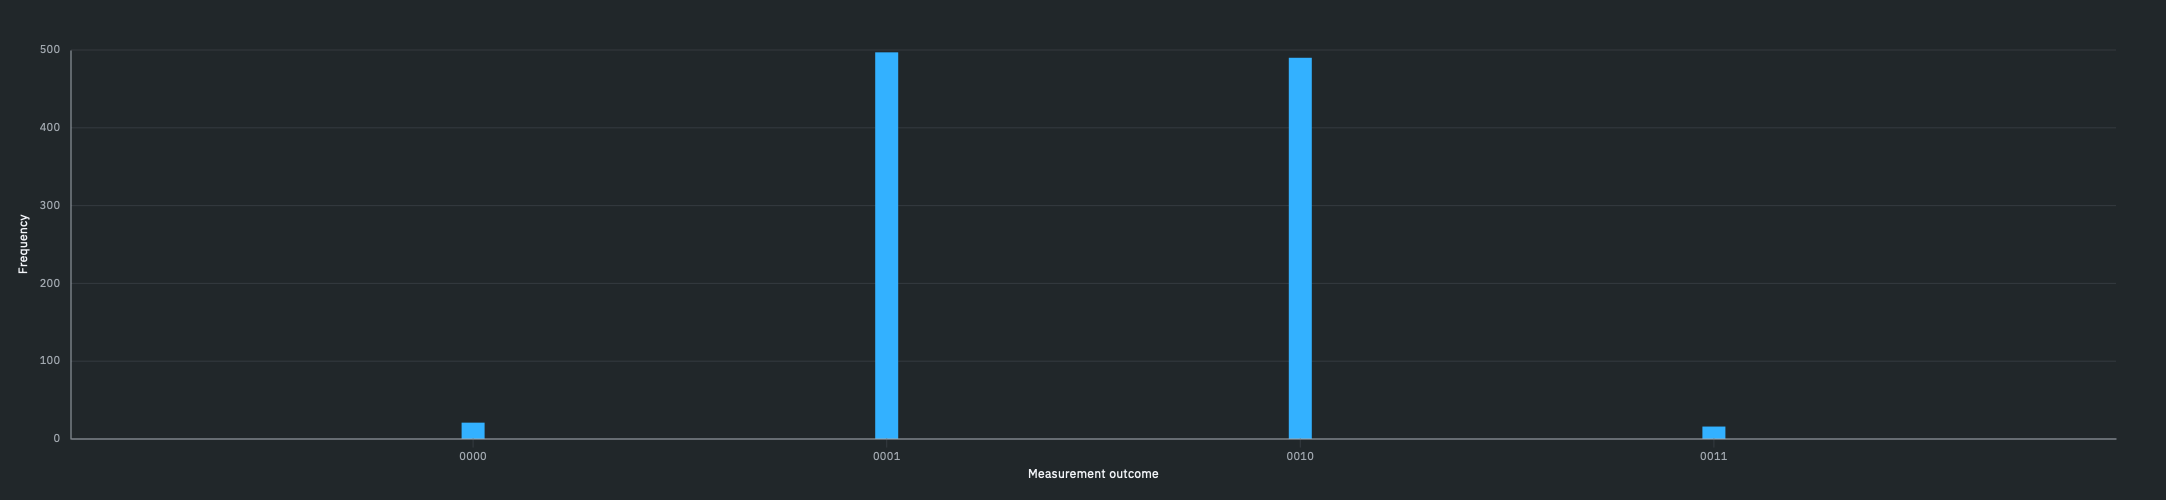
\includegraphics[width=0.9\textwidth]{q4_b_sherbrooke.png}
      \captionof{figure}{Screenshot of the results from the IBM Quantum Composer on IBM Sherbrooke.}
      \label{fig:4b_sb}
    \end{minipage}
  \end{proof}
\end{solution}

\begin{solution}[label=ques:4c]
  \begin{question}
    Calculate the empirical TV distance of the theoretical output distribution of the circuit from the distribution produced by the quantum computer. Show your work.
  \end{question}
  \tcblower{}
  \begin{proof}[Solution]
    The theoretical output distribution will be $\{0, 0.5, 0.5, 0\}$. The output ditribution from the statevector is $\{0, 0.508, 0.492, 0\}$ and from IBM Sherbrooke is $\{0.020, 0.479, 0.485, 0.016\}$. Therefore, the TV distance between the theoretical distribution and statevector distribution is $0.008$ and between the theoretical distribution and IBM Sherbrooke distribution is $0.036$.
  \end{proof}
\end{solution}
